 \documentclass[10pt,letterpaper]{article}
\usepackage[top=1in,bottom=1in,left=1in,right=1in]{geometry}
\usepackage{datetime}
\usepackage{natbib}      % http://merkel.zoneo.net/Latex/natbib.php
\usepackage{palatino}
\usepackage{verbatim}
\usepackage[normalem]{ulem}
\bibpunct{(}{)}{;}{a}{,}{,}

\usepackage{array}

\usepackage{chngpage}
\usepackage{stmaryrd}
\usepackage{amssymb}
\usepackage{amsmath}
\usepackage{graphicx}
\usepackage{lscape}
\usepackage{subfigure}
\usepackage[usenames,dvipsnames]{color}
\definecolor{myblue}{rgb}{0,0.1,0.6}
\definecolor{mygreen}{rgb}{0,0.3,0.1}
\usepackage[colorlinks=true,linkcolor=black,citecolor=mygreen,urlcolor=myblue]{hyperref}

\newcommand{\bocomment}[1]{\textcolor{Bittersweet}{BO says: #1}}

\newcommand{\ignore}[1]{}
\newcommand{\transpose}{^\mathsf{T}}
\newcommand{\inner}[1]{\langle #1 \rangle} 
\newcommand{\smallsec}[1]{\noindent \textbf{#1\ }}
\newcommand{\cmd}[1] {{\color{blue}\texttt{#1}}}

\newcommand{\solution}[1]{{\color{myblue} \emph{[Solution:} 

#1 

\emph{End solution]}}}
\newcommand{\solutionnote}[1]{{\color{myblue} \emph{[Note:}

#1 

\emph{End note]}}}
\newcommand{\points}[1]{{\color{mygreen}\emph{[#1]\ \ }}}

\newcommand{\aone}{\diamondsuit}
\newcommand{\atwo}{\heartsuit}
\newcommand{\bone}{\triangle}
\newcommand{\btwo}{\Box}
\newcommand{\myand}{\ \land\ }
\newcommand{\myor}{\ \lor\ }
\newcommand{\mynot}{\lnot}

\title{
  Homework 4 \\
  \Large{CMPSCI 370 Spring 2019, UMass Amherst} \\
  \Large{Due: April 10, 11:55 PM} \\
  \Large{Instructor: Subhransu Maji} \\
  \Large{TA: Tsung-Yu Lin}
}

\settimeformat{ampmtime}
\date{}
\begin{document}
\maketitle

\renewcommand\thesubsection{\thesection.\alph{subsection}}


\section*{Guidelines}

\paragraph{Submission.} Submit your answers via Gradescope that includes a pdf with your solutions and source code. You have a total of 5 late days for all your homework assignments which you can use in any way you like. However note that delay by even one minute counts as a full late day and submissions beyond the late days will not be given \emph{any} credit. Please contact the instructor and obtain permission ahead of time if you seek exceptions to the policy.

\paragraph{Plagiarism.} We might reuse problem set questions from previous years, covered by papers and webpages, we expect the students not to copy, refer to, or look at the solutions in preparing their answers. We expect students to want to learn and not google for answers. Any instance of cheating will lead to zero credit for the homework, and possibly a failure grade for the entire course.

\paragraph{Collaboration.} The homework must be done individually, except where otherwise noted in the assignments. 'Individually' means each student must hand in their own answers, and each student must write their own code in the programming part of the assignment. It is acceptable, however, for students to collaborate in figuring out answers and helping each other solve the problems. We will be assuming that you will be taking the responsibility to make sure you personally understand the solution to any work arising from such a collaboration.

\paragraph{Matlab requirements.} The code should work any Matlab version ($\geq$ 2011a) and relies on the Image Processing Toolbox for some functions.

\paragraph{Python requirements.} We will be using Python 2.7. The Python starter code requires \cmd{scipy}, \cmd{matplotlib} and \cmd{pillow} for loading images and \cmd{numpy} for matrix operations (at least v1.12). 
If you are not familiar with installing those libraries through some package manager (like \cmd{pip}), the easiest way of using them is installing \href{https://conda.io/docs/user-guide/install/index.html}{Anaconda}. Contact the course staff if you are having trouble installing these.

\paragraph{Using other programming languages.} We made the starter code in Python and Matlab. You are free to use other languages such as Octave or Julia with the caveat that these will not be supported by the course staff.

\newpage

\section{Scale Invariant Feature Transform}

Answer these questions in one or two sentences.
\begin{itemize}
\item \textbf{(2 points)} What are the advantages of  blob detection over the Harris corner detection?
\vspace{1.5in}

\item \textbf{(2 points)} How is rotation invariance achieved in SIFT features?
\vspace{1.5in}

\item \textbf{(2 points)} When can matching patches using sum-of-squared-differences between the vector of pixel values fail? List two scenarios when the pixel values can change significantly.
\vspace{1.5in}

\item \textbf{(2 points)} List two ways how the SIFT descriptor provides robustness during feature matching?
\vspace{1.5in}
\end{itemize}

\newpage
\section{Panoramic Image Stitching}
In this part you will implement a simple panoramic image stitching algorithm. The input to the algorithm are two images which are related by a unknown translation and scale \cmd{(tx, ty, s)}. Your goal is to estimate this transformation using feature matching and RANSAC to produce a combined image. Recall that the overall steps in the alignment algorithm are:

\begin{enumerate}
\item Detect corners in each image (code provided/previous homework).
\item Extract features at each corner.
\item Match features based on distance in feature space.
\item Use RANSAC to estimate transformation.
\item Transform the second image using the estimated transformation (code provided).
\end{enumerate}

The codebase contains an implementation of Step 1 and Step 5. You are welcome to use your own implementation of the Harris corner detector, but in case you decide to use the provided \cmd{detectCorners()} function the details are described later. 

The entry code for this homework is in the file \cmd{stitchImages}. The code loads two images as seen in Figure~\ref{fig:examples} provided in the latex folder. There are multiple variants of the right image, numbered 1 through 5, corresponding to different amount of translations and scaling. 
For this homework all the image pairs can be perfectly aligned with by scaling and translation.
In reality panoramic stitching may require solving for a general affine transformation. You are welcome to implement this for extra credit (see the lecture slides for details). 

Your goal is to implement the all the steps in the alignment algorithm, report the estimated transformation, as well present visualizations of matches and the final merged image. 
The steps are described next.


\begin{figure}[h]
\centering
\begin{tabular}{cc}
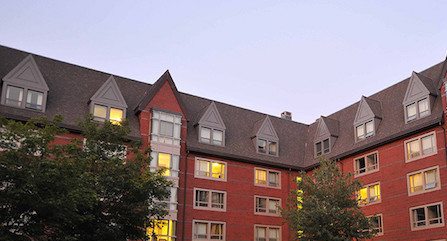
\includegraphics[scale=0.5]{../data/umass_building_left.jpg}&
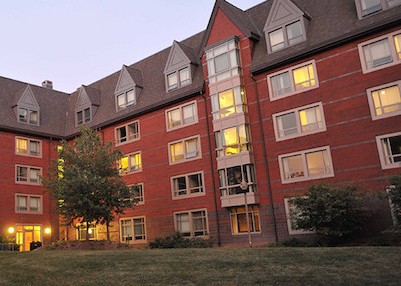
\includegraphics[scale=0.5]{../data/umass_building_right1.jpg} \\
umass\_building\_left.jpg & umass\_building\_right1.jpg 
\end{tabular}
\caption{\label{fig:examples} Input images for the image stitching.}
\end{figure} 

\subsection{Detect corners [0 points]}
The first step is to detect corners in each image independently. You already implemented this in the previous homework, but the codebase provides an implementation in case you want to use this. The provided function \cmd{c = detectCorners(I, isSimple, w, th)} returns a single matrix $c$ which has three rows \cmd{c = [cx; cy; score]} containing the x coordinates, y coordinates and the score. Note that you have to change your homework 3 code slightly to return all three outputs as a single array. This makes it convenient to pass these as input to the feature extraction and matching code. This code finds corners by setting \cmd{isSimple=false, w=1.5, th=0.0005}. It also keeps the top 200 corners for computational efficiency.


\subsection{Feature extraction [20 points]}
The next step is to implement a function \cmd{f = extractFeatures(im, c, r)} that extracts a vector of raw-pixel values from \cmd{im} centered at each corner in \cmd{c}. The basic steps in the process are:
\begin{enumerate}
\item Convert color image to gray
\item For each center \cmd{cx} and \cmd{cy} in the corner array \cmd{c}, extract a patch of radius \cmd{r} centered at the \cmd{[cx,cy]} from the gray-scale image. Reshape the patch to a vector (using the (:) operator or reshape function) to obtain a feature of size $(2r+1)^2$. The scheme is illustrated in Figure~\ref{fig:feat}. 
You can pad the image by r pixels to extract patches near the edges (using \cmd{padarray()}/\cmd{np.pad()} command), but be careful to take into account the shift in the positions of the corners due to padding.
\end{enumerate}

The input is \cmd{c = 3$\times$N}, where \cmd{N} is the number of corners, and the output is a matrix \cmd{f = d$\times$N}, where \cmd{d = $(2r+1)^2$} is the feature dimension. The code in \cmd{stitchImages.m} file calls this function to extract features from both the images using the detected corners in the previous step.

\begin{figure}[h]
\centering
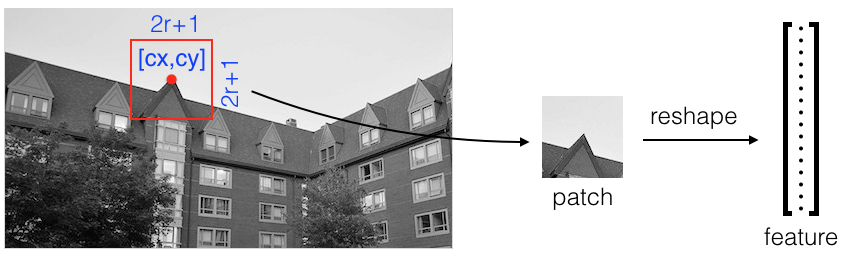
\includegraphics[width=0.9\linewidth]{patchFeatures.png}
\caption{\label{fig:feat} Patch feature of radius \cmd{r} extracted from a grayscale image at a point \cmd{[cx,cy]}.}
\end{figure}

\subsection{Computing matches [20 points]}
The next step is to compute matches between the two sets of features. 
Implement the function \cmd{matches = computeMatches(f1,f2)} that returns the best match of each feature \cmd{f1} to \cmd{f2} using the smallest sum-of-squared-differences as the distance measure. 
The input are two matrices \cmd{f1=d$\times$N} and \cmd{f2=d$\times$M} and the output is a array of size \cmd{N$\times$1} where each entry \cmd{matches(i)$\in {1, \ldots, M}$} is the closest feature in \cmd{f2} to the $i^{th}$ feature \cmd{f1(:,i)}.
As an illustration say the first feature in \cmd{f1} matches to the 10$^{th}$ feature in \cmd{f2}, then we have \cmd{matches(1) = 10}. Features that are not matched to any should be assigned a \cmd{matches(i) = 0}. Note that this can happen if you implement the ratio-test to remove unreliable matches.

Once you have implemented this function you can visualize the matches using the \cmd{showMatches(im1, im2, c1, c2, matches)} function provided in the codebase. Figure~\ref{fig:all} shows the output of my implementation for reference.
\begin{figure}[h]
\centering
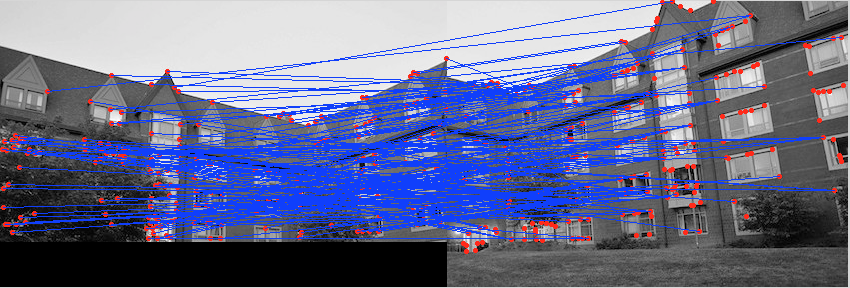
\includegraphics[width=0.9\linewidth]{allmatches.png}
\caption{\label{fig:all}All matches between features extracted from the corners.}
\end{figure}

\subsection{Estimating transformation using RANSAC [40 points]}
The matching in the previous step is noisy and contains many outliers. 
Using RANSAC you can estimate the transformation that agrees with most matches. In particular the coordinates of the second image $(x', y')$ are related to the coordinates of the first image by an unknown scale $s$ and translation $(t_x,t_y)$:
\begin{eqnarray}
x' &=& sx + t_x, \\
y' &=& sy + t_y.
\end{eqnarray}

You need at least two matches to estimate the scale and translation. For example, say you have two points $(x_1, y_1)$ and $(x_2, y_2)$ in the first image that get matched to $(x'_1, y'_1)$ and $(x'_2, y'_2)$ in the second image. The coordinates of the points are related as:
\begin{eqnarray}
x'_1 &=& sx_1 + t_x,\\
y'_1 &=& sy_1 + t_y, \\
x'_2 &=& sx_2 + t_x,\\
y'_2 &=& sy_2 + t_y.
\end{eqnarray}
From this one can obtain the scale $s$ as:
\begin{equation}
s = \frac{\sqrt{(x'_1-x'_2)^2 + (y'_1-y'_2)^2}}{\sqrt{(x_1-x_2)^2 + (y_1-y_2)^2}}.
\end{equation}
The translation parameters $(t_x,t_y)$ can be estimated by substituting the estimated $s$ in the above equations. 
You can also directly estimate all the three parameters by solving the above system of linear equations. See lecture slides for details.

Note that the estimated translation depends on the coordinate system of the images. The provided code for the corner detector assumes the top-left corner of the image is the origin, with x and y coordinates increasing from left to right and top to bottom respectively. Using this coordinate system the corresponding points in the right image are shifted to the left and up (the camera motion is to the right and down), so the estimated \cmd{tx} and \cmd{ty} should both be negative.

Given a transformation $T$, you can map a point in the second image to the first image using:
\begin{eqnarray}
T(x'_1) &=& (x'_1 - t_x)/s,\\
T(y'_1) &=& (y'_1 - t_y)/s,
\end{eqnarray}
and check if it is close to its match in the first image (estimated in the earlier step) to decide if it is an inlier; For example if the squared Euclidean distance between the two is less than some threshold $\tau$:
\begin{equation}
\left(x_1 - T(x'_1)\right)^2 + \left(y_1 - T(y'_1)\right)^2 < \tau.
\end{equation}
The RANSAC algorithm should return a transformation that has the highest number of inliers. Note that the threshold $\tau$ has to be set experimentally. You may also estimate the inliers by transforming the points from the first image to the second and checking if they are close to the destination. However since in the examples the first image is fixed, transforming the features from the destination to the source will allow you to keep the value of $\tau$ fixed across all image pairs. 

Implement the function \cmd{[inliers, transf] = ransac(matches, c1, c2)}. Here \cmd{inliners} is the indices of the inliner matches, and \cmd{transf = [tx, ty, s]} is the estimated transformation from \cmd{c1} to \cmd{c2}, i.e., the estimated shift and scale of the right feature points with respect to the left feature points.

After implementation of this step you can visualize the inlier matches using the \cmd{showMatches} function (see \cmd{stitchImages} for details). Figure~\ref{fig:inliers} shows the output of my implementation for reference.

\begin{figure}[h]
\centering
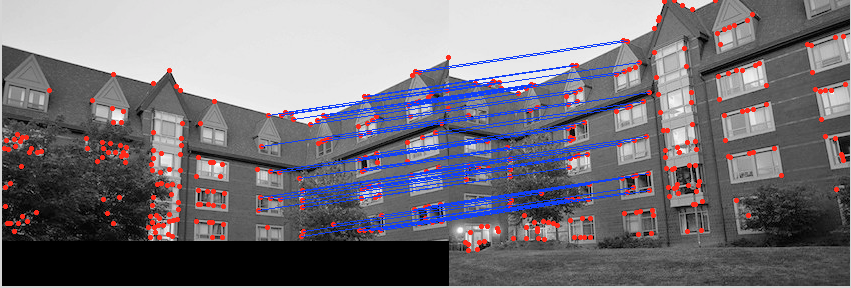
\includegraphics[width=0.9\linewidth]{inliers.png}
\vspace{-0.1in}
\caption{\label{fig:inliers}Inlier matches between features computed using RANSAC.}
\vspace{-0.1in}
\end{figure}

\vspace{-0.1in}
\subsection{Visualizing the stitched image [0 points]}
Merge the images using \cmd{mergeImages(im1,im2,transf)} function provided in the codebase. The images should align well in the overlapping region as shown in Figure~\ref{fig:result}.

\begin{figure}[h]
\centering
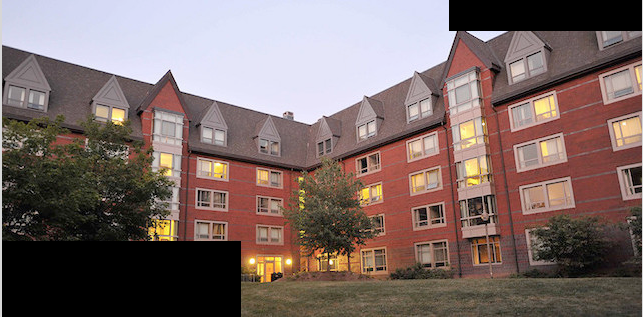
\includegraphics[width=0.88\linewidth]{result.png}
\vspace{-0.1in}
\caption{\label{fig:result}Result of stitching the two 
images}
\vspace{-0.1in}
\end{figure}

\subsection{What to submit?}
Keeping the \cmd{im1} same run your algorithm for various \cmd{im2} corresponding to each of the five right images. These images are included in the homework folder.
For this part of the homework your submission should include:
\begin{itemize}

\item The estimated transformation \cmd{[tx,ty,s]} and the number of inliers for each of the provided images in a tabular form (see below).

\begin{table}[h]
\centering
\begin{tabular}{c|c|c|c|c}
im2 & tx & ty & s & \#inliers\\
\hline
umass\_building\_right1.jpg & & & &\\
umass\_building\_right2.jpg & & & &\\
umass\_building\_right3.jpg & & & &\\
umass\_building\_right4.jpg & & & &\\
umass\_building\_right5.jpg & & & &\\
\end{tabular}
\caption{Estimated transformation.}
\end{table}
\item The outputs of each step, i.e., matches (Figure~\ref{fig:all}), inliers (Figure~\ref{fig:inliers}), and the stitched image (Figure~\ref{fig:result}), for each of the five image pairs.
\item The code for the files \cmd{extractFeatures.m, computeMatches.m} and \cmd{ransac.m} (or the python variants)
\end{itemize}

\subsection{Tips}
Here are some tips:
\begin{itemize}
\item Start with im2=umass\_building\_right1.jpg which will be easiest to align since the two images are roughly at the same scales, i.e., $s\sim1$, and the transformation is a pure translation.
\item The images 1 through 5 are of progressively smaller scales. Since your feature extractor is not scale invariant, matching features across scales will not be as robust leading to fewer inliers. 
Accordingly you may have to run RANSAC for more iterations for some of these images.
SIFT features are better suited for this since the features are scale invariant.
\item RANSAC algorithm is randomized so your results will be slightly different each time you run it.
To make debugging easier you may fix the random seed to make the algorithm deterministic.
\item Feel free to explore the parameters of the corner detector, the number of features used in matching, and the patch radius used for feature extraction. The default values work well for all the provided images, but depending on your implementation other values may give you more robust results.
\item You will know when your results are correct as the images will line up as shown in Figure~\ref{fig:result}.
\item Compare this approach to the Prokudin-Gorskii alignment procedure in Homework 1. Try running your code on those images to see if your RANSAC produces the same alignments as the brute-force search.
\end{itemize}

\section{Submission and rubric}

\begin{itemize}
\item Follow the outline on Gradescope for your submission. 
\item A fraction of the points for each coding assignment will be for
  readability and efficiency of your code. Thus it is important to
  properly document parts of the code you implemented.
\end{itemize}

\end{document}
